High-resolution, high-throughput microscopy has opened possibilities for biological analysis that were inconceivable only a few short years ago, but the methods by which to analyze these data remain largely lacking. While heroic efforts have been made to use both standard thresholding methods as well as newer machine learning-powered methods to simplify and automate image processing, these approaches are often somewhat limited by the range of purposes for which they were designed and tested. While the open source nature of many of these approaches facilitates adaptation, this is both technically beyond the skillset of many scientists and impeded by, at best, variable quality documentation. Additionally, many of the tasks that experimenters seek to do are both relatively simple and highly repetitive but they are often unaware of the means by which to cut down on manual processing time in order to economize their time and energies. These scripts are a combination of automation scripts that will process particular image types into smaller and more informative images (compression of Z-stacks, time-series, etc.) and those meant for analysis of image data (pixel intensity distribution across an image, bacterial burden within larval zebrafish). While none of these are of the caliber to open entirely new methods of analysis, I hope they are a catalyst for others in the zebrafish community at large to explore the potential for computational automation to save time and frustration in the process of analyzing often thousands of very large, data-rich images.

All of the scripts in their latest versions will be able to be found in perpetuity at \url{http://github.com/jaredbrewer/image-analysis}. A static version of these has been created at Zenodo (\url{https://doi.org/10.5281/zenodo.7036029}). Scripts at the end for RNA sequencing analysis are available at Zenodo (\url{https://doi.org/10.5281/zenodo.6981721}). 

\section{FIJI/ImageJ}\label{fiji}

ImageJ was first developed in embryo in the 1980s as a means of viewing scientific images on the Mac, but matured into the program we know today in the 1990s when it was ported to Java. The original ImageJ1 is still developed and maintained today and serves as the foundation of its functional successor, FIJI. \underline{F}iji \underline{I}s \underline{J}ust \underline{I}mageJ is essentially ImageJ2 bundled with a set of useful plugins that aid in visualizing and analyzing scientific imaging data. Preeminent among these bundled plugins is a library of programming languages that can be used to interface with the underlying Java-based APIs that make FIJI function. Among the options, Python is likely the most widely known and written programming language among biologists and this opens up a great deal of potential for object-oriented programming centered on the analysis of images. 

The default language in ImageJ, the ImageJ1 Macro language (.ijm), is approximately based around Java but lacks defined sets of methods (for most purposes) and objectification, has difficulty with interfacing with file systems, and exposes a great deal of underlying computer logic to the user. Take, for instance, the procedure for writing a \textit{for} loop:

\begin{code}
\begin{minted}{java}
for (i = 0; i < 10; i++) {
    print("Hello");
}
\end{minted}
\end{code}

\begin{code}
\begin{minted}{python}
for i in range(1:10):
    print("Hello")
\end{minted}
\end{code}

The former example, written in the IJ1 macro language, exposes the user to looping over a set of indices from 0 to 10 and incrementing with each loop, uses curly braces to define the boundaries of the loop block, and requires each line to end with a semicolon. These are all standards features of many popular programming languages, but for FIJI, the key is to be as legible of a programming language as possible since the writers of most of these macros are \textit{not} software engineers. Python, by contrast, increments for the user and will increment through an entire set of objects without needing to know how many objects are present. Blocks of code are delimited by spaces or tabs, so the relative location of the code on the line is informative as to what it relates to. Additionally, Python has well-studied and well-defined object types with specific associated methods that translate between all versions of Python. The benefits of the Python community only add to the value proposition of learning and using Python both generally and within ImageJ.

Not only this, but to loop through directories of files, the ImageJ macro language struggles even further, with little awareness of file structures or regular expressions whereas Python can trivially fetch lists of files by user-defined patterns from mixed directories and even search through subdirectories recursively.
 
\section{Python}\label{python}

As alluded to, Python is a dynamically typed high-level programming language that is widely used for generating automation scripts of all varieties in addition to web server backend applications, data science, and even game creation \citep{vanRossum1995}. The advantages of Python are derived from the enormous community of developers who use Python and who continue to develop it as a language. In data science, the utility of pandas and numpy are unmatched and these alone make Python a language worth learning for any molecular biologist in the analysis of their quantitative data. Throughout this work, I have used Python both within the FIJI/ImageJ interpreter (which is based on Jython version 2.7.2) and via CPython 3.11, the standard distribution of Python, in the Terminal. While Jython is nominally different from standard Python, when written appropriately, it is simple enough to write version-universal code within the relatively narrow confines of what I have sought to accomplish thus far with it.

One of the key developments in the field of FIJI and Python is the release of PyImageJ, a complete API interface between CPython and ImageJ2, written in Python \citep{Rueden2022}. Going forward, it will be useful to reimagine some of these scripts and approaches to utilize the PyImageJ-defined API, as this is clearly the future of scripting in FIJI. Use of the image viewer in an \textit{ad hoc} fashion is likely superior to an image-first approach for many tasks and PyImageJ cuts a lot of the unfortunate overhead from the graphical elements of FIJI. Unfortunately, such a translation is nontrivial as the command structure and imports have changed quite dramatically and in ways that are not as well documented as the base API. However, such an implementation allows FIJI/ImageJ to make use of pandas, numpy, and OpenCV in Python, making for a more complete data science package and streamlining data collection and processing in a single language. 

\subsection{Napari}

While FIJI/ImageJ have served as the key to the analyses presented both here and in \autoref{chap3}, it is not the only image analysis software available. An alternative, written in pure Python, is napari, which is in the middle stages of alpha testing as of this writing \citep{napari}. While not yet feature complete, it is a lightweight alternative to FIJI and, with proper optimization, can likely outperform FIJI in the long run. By shedding dependence on Java, memory management and performance are able to be improved while the lowest-level image processing can be done in C invisible to the end user. At the present time, however, FIJI seems to be the most robust and widely accepted option and will likely remain so for the conceivable future. A bridging option, \textit{napari\hyp{}imagej} is in the works and promises to dramatically expand the napari feature set, but does not aid in napari independence from Java or older modalities.

\section{R}\label{R}

As previously detailed (\autoref{meth:R}), R is a convenient and easy-to-learn object-oriented statistical programming language. This language has made a monumental contribution to data science and is used extensively throughout this work to analyze and visualize the resulting datasets. While less extensively used in this segment than Python, it is key to a lot of further analyses and is exhaustively used for all of the visualization seen in \autoref{chap3}. Many of these same functions can be executed in Python, but I attempt to utilize the best tool for a given task at a given time and R is often the best, most flexible way to work with arrays and data frames.

\section{Maximum-Intensity Projection and Composite Image Generation}\label{mippers}

The fundamental premise of the ImageJ macro system is to simplify repetitive tasks to free up user time for higher forms of analysis and the default language (the ImageJ1 macro language) makes it easy to write procedural operations to be done on single images, but is difficult to scale to whole directories of images or accept various types of user input. I have thus developed a set of scripts that allow the user to rapidly generate maximum-intensity projections from sets of images and then generate composite images. This often condenses hundreds of megabytes of data into $<$30 MB, makes for more flexible image viewing and understanding, and allows the images to be opened in essentially any number (many hundreds to thousands) on any personal computer. These procedures are also internally memory managed, allowing them to run on most personal computers indefinitely to process the sometimes thousands or tens of thousands of images that can be generated over the course of an experiment with multiple wavelengths, Z stacks, XY positions, and times\footnote{If you have 4 channels across 48 stage positions, capturing every 30 minutes for 48 hours, you would have 18,432 individual images based on Metamorph's file saving structure; this can clearly get out of hand very quickly.}. In our lab, we primarily use output files from epifluorescent Zeiss microscopes, which generate .czi files and from Metamorph connected to a custom spinning disk confocal system, which generates .tiff files.

The maximum intensity projection is an extremely common way of condensing multidimensional images into a single two-dimension representation by finding the brightest pixel at every XY position and accepting it as the most ``in focus'' pixel. The success of this depends on images being properly exposed, but in most instances will generate a reasonably sharp image ready to be quantitated or presented. In any case, data spanning multiple Z stacks requires some degree of integration to be usefully presented to others or manual scanning through libraries of hundreds of images and these pipelines will facilitate that type of visualization at scale.

\begin{code}
\caption{This script allows the user to open as many files as their memory allotment will allow and then to Z project them one at a time with custom start and end positions. This ability often generates cleaner, sharper images by individually selecting the lowest and highest in-focus frames, but necessarily takes more time than a more automated approach.}
\label{slowmanmip}

\inputminted[breaklines,frame=single,fontsize=\small]{python}{source/manMIPper.py}

\end{code}

The use of \autoref{slowmanmip} is to process a set of already opened images and generate maximum intensity projections from these and, optionally, save them back into the directory that they came from. This relatively simple set of GUI-guided processes allows the user to, in two clicks, accomplish a task that previously would have required a great deal of menuing to accomplish. The goal is narrow, but this execution is extremely useful when working through large numbers of images. This is readily adaptable to any workflow as it has no features specific to a given image type or contents, so could easily be reused by many different individuals for their own purposes, like the subsequent scripts to process maximum intensity projections by other modes.

This script will first open a GUI with a simple set of inputs: the minimum and maximum slices that the user would like to use in creating the Z projection. This GUI is a ``non-blocking'' GUI, and can thus be opened in advance of deciding which slices to use -- a convenience that frees the user from having to remember which slices were the best (\autoref{figure:mipgui}). 

\begin{figure}
\centering
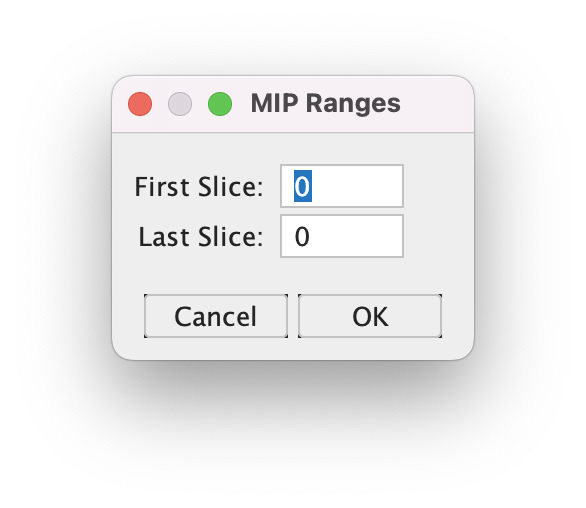
\includegraphics[height=2in]{images/mipgui.png}
\caption{This is the entire graphical user interface and inputs required to run this script: the script asks for the top and bottom slices from the image of interest and then runs the rest of the script.}
% Provide a label so we can cross\hyp{}reference it from the tex
\label{figure:mipgui}
\end{figure}

The internal logic of this macro seeks to minimize opportunities for user-derived error by checking whether the values provided are logical. The top slice needs to have a value greater than the bottom slice\footnote{This is not a technical requirement -- indeed, the ZProjector function itself can take these argument in either order, but it seemed to me that if the numbers are put in the wrong order that this suggested a user error in input and was not intended.}, but if both are left as the default (0), then it will create a maximum intensity projection across the whole image. This allows it to be a single-click convenience button for performing this operation on any number of images, although other options presented later are likely to be better choices for this. Additionally, if the top value is set to a number greater than the total number of slices, then it provides an error to the user. This adds some safety to the operations and prevents unintended operations, although the risk of data corruption is essentially non-existent. 

This, like many of the scripts further on, incorporates memory management to improve FIJI stability and prevent runaway memory leakage from Java, which very inefficiently clears out unused sectors even when the image has been closed. Thus, approximately one in every eight runs, the macro will run garbage collection to free up memory which can allow for more extended uptime for FIJI in the process of doing numbers of images far in excess of nominal memory space; however, for this, I could recommend looking to \autoref{fastmanmip}, which is written for essentially unlimited images in any reasonable memory buffer capacity.

A future version will incorporate a one-time checkbox that will allow the user to choose whether they would like to automatically reopen the dialog box for each image that they have open currently. If it is selected on the first run, it will then open for every subsequent image until cancelled. This should streamline these processes and further minimize clicks-per-operation, which should be the primary goal of these sorts of automation macros.

\begin{code}
\caption{A low overhead version of the manual maximum intensity projection script described above. Instead of opening all of the images first and then running the script, the script will processively open unanalyzed images one at a time and periodically garbage collect, allowing for entire directories to be processed at once on most reasonably modern computers.}
\label{fastmanmip}

\inputminted[breaklines,frame=single,fontsize=\small]{python}{source/fast_manMIPper.py}

\end{code}

\autoref{fastmanmip}, while not always the correct choice depending on user preferences and system capabilities, is much less memory hungry than the original version above, but typically results in slightly slower overall operations due to the delay in opening images. If the images are on fast internal storage, then this is certain to be faster than \autoref{slowmanmip}, but when reading from external storage, the I/O limitations will likely make it faster to open all of the images prior to processing unless system memory is severely limited. Nevertheless, the nature of this makes it very generally useful on older systems.

The user interface prompts the user to provide a directory that contains all of the desired images and provide the file extension from a pre-populated list or provide their own (\autoref{figure:automipgui}). These are the only user-inputs required to get this processing started; from there, a dialog box will open after each image has been opened requesting the first and last slices for maximum intensity projection, which can vary from image to image.

\begin{figure}
\centering
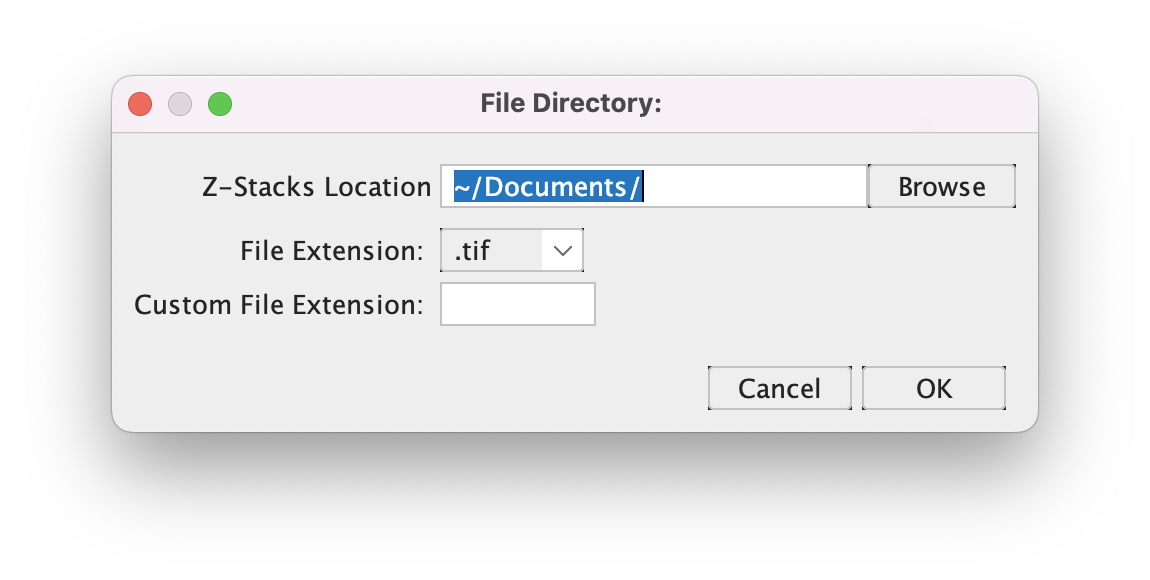
\includegraphics[width=3in]{images/automipgui.png}
\caption{This GUI pop\hyp{}up asks the user for the file directory that they would like to process and will process only the images directly in that folder; it also asks for the file extension so that it will only process the desired images in case the user has additional data in that folder.}
% Provide a label so we can cross\hyp{}reference it from the tex
\label{figure:automipgui}
\end{figure}

The internal logic of this script prevents the user from accidentally processing the same image more than once; this allows the processing to be done in session over time rather than all at once. The script looks for a file with the expected naming structure for the output and, if it is found, removes the original file from the list of inputs. This also hedges against FIJI crashing or other errors. To do an image again due to some user input error, the user can either use \autoref{slowmanmip} or remove the projection from the directory and the script will then allow it to be processed again. 

This script also utilizes an identical memory management approach to the previous, which has allowed this to function over thousands of images at once. This offers a distinct advantage over manual memory management approaches that have to be used during manual processing and the requirement to open all of the images beforehand, a process inherently limited by available system memory.

\begin{code}
\caption{This script can be used in instances where the first and last stacks of a desired Z projection span the entire set of stacks provided. It will process an entire directory of images together and output the result into a subdirectory of the original.}
\label{bulkmip}

\inputminted[breaklines,frame=single,fontsize=\small]{python}{source/bulkMIPper.py}

\end{code}

While the previous scripts have expected user input for each image, the skilled microscopist can select top and bottom slices that will suffice for generating Z projections during imaging itself. This means that the first and last slices of the projection are typically the first and last slices of the images \textit{in toto}. This script takes a directory of images as an input and will perform total maximum intensity projections on all of them and save in a new subdirectory. After observation, any that seem incorrect can then be processed with one of the preceding scripts, especially \autoref{slowmanmip}. 

The only prompting from the user is to provide a directory and file extension, just like \autoref{fastmanmip}. As a result of the lack of user intervention during processing, the internal logic of this script is much simpler and will simply perform top-to-bottom projections of each of the files in the directory and then save them in a subdirectory of the original directory provided. This operation can easily processing hundreds of images per minute and cuts processing time down dramatically -- whereas it can take 10-15 seconds per image doing it strictly by GUI, it can now do dozens to hundreds of images in that same time period. Not having to physically show the image also improves performance, although the user can opt to have it show the projections if desired by simple modifications to the code. A future version should incorporate an option to turn this on or off within the GUI; it should be reasonable for most computers to be able to show the maximum intensity projections for at least a few hundred images, although selecting such an option will come with some performance penalty.

\begin{code}
\caption{An interface to functions allowing slices in a Z-stack to be kept or removed as desired through function calls. This can integrate into other workflows and be connected to the previous scripts through higher-order wrappers.}
\label{reslicer}

\inputminted[breaklines,frame=single,fontsize=\small]{python}{source/reSlicer.py}

\end{code}

FIJI/ImageJ comes with a built-in option to keep and remove particular slices (Image $>$ Stacks $>$ Tools $>$ Slice Keeper / Slice Remover), but the native plugin does not readily fit into object-oriented programming pipelines like those used by Python and Java; it is very operational toward the currently open image and does not have a well-defined API. Thus, I have adapted the underlying logic of these plugins to be wrapped in various other scripts through calls to the defined functions, \textit{sliceKeeper} and \textit{sliceRemover}. For instance, this allows calls to the maximum intensity projection plugins to be funneled into this plugin to simultaneously generate the kept slices as well as the maximum intensity projection of those kept slices for some useful improvements to data integrity. 

Integration of this as in import into the other scripts previously described with an additional option would be an intelligent way of making use of this plugin; it also reveals the many opportunities to expand upon and add functionality to the previously detailed plugins based on user needs. The addition of saving the exact slices used to generate maximum intensity projections along with some sort of metadata seems like it would improve data integrity in a meaningful way, although at the cost of increased storage requirements.

\section[Surface Plot Analysis for Cellular Distribution of Labeled Proteins]{Surface Plot Analysis for Cellular Distribution of Labeled Proteins\footnote{Taken from personal contributions to \citet{Saelens2022}.}}

The distribution of a protein across the cell body can indicate changes in function of the protein and alterations in cell behavior, but analysis of such changes is not quite trivial. There are methods for drawing lines and plotting fluorescence intensity, but this fails to integrate the entire cell in three dimensions in to the analysis as it proves to be only one dimensional along that line. To analyze the distribution of ARPC2 in BLaER1 macrophages during \textit{M. tuberculosis} infection, I developed a novel analysis pipeline that integrated the 3D Surface Plot plugin of ImageJ. This pipeline takes a raw image, isolates the desired channel, opens it in 3D Surface Plot for visualization, and then takes the user-generated output of 3D Surface Plot to find the maximum fluorescence along the longest axis of the cell. As this analysis is designed for macrophages, which can develop long spindles, this allows for quantitative proximal/distal differences in the localization of a protein to be determined.

\begin{code}
\caption{A script to isolate a single cell within a frame.}
\label{isolator}

\inputminted[breaklines,frame=single,fontsize=\small]{python}{source/autoIsolator.py}

\end{code}

The first step of this pipeline is to isolate the cell using some reference channel, which can also be the channel you are measuring if necessary, although I would recommend using some sort of pan-cytosolic or plasma membrane marker to more thoroughly mark the outline of the cell and to use that instead. The script presents a simple GUI (\autoref{figure:spgui}) and allows the user to select the needed parameters and will then process entire folders of images into isolated cells in a single channel. A missing feature is that it needs to be able to isolate each cell from images that contain more than one cell, to save the user time on isolating cells in their own separate files by hand. This could conceivably be done by integrating logic around coping ROI contents into new images, but that is a work-in-progress at this time.

\begin{figure}
\centering
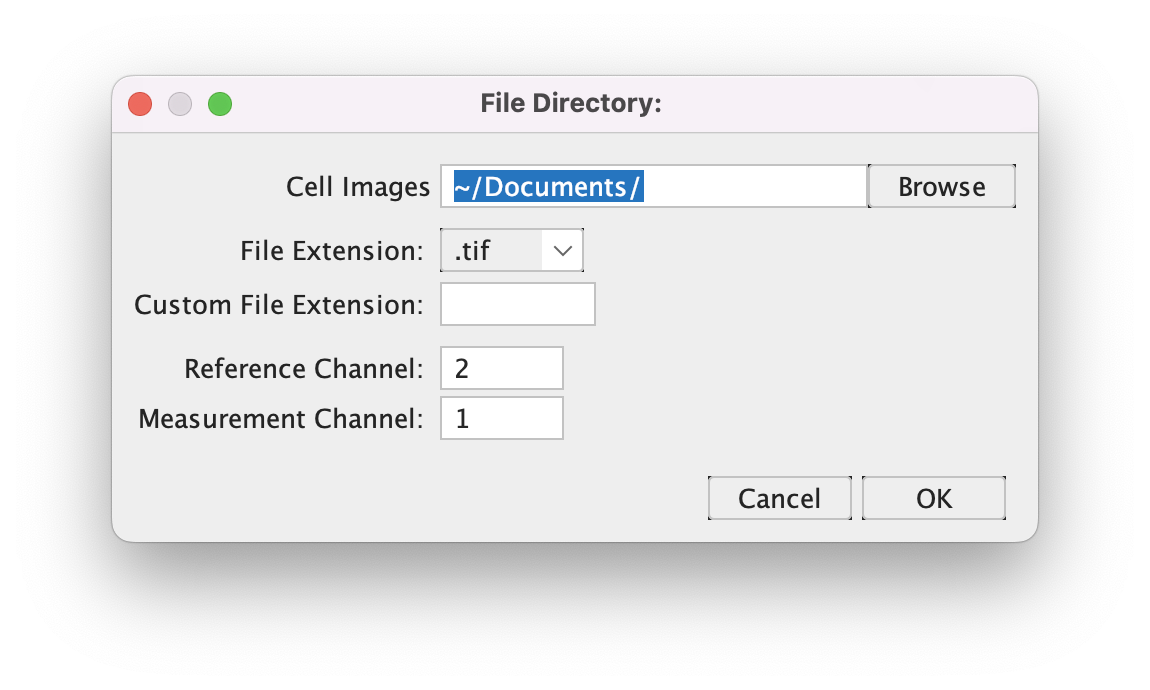
\includegraphics[width=3in]{images/spgui.png}
\caption{The user needs to provide a number of factors to allow for this function to operate properly: a file directory with the images that should be processed, the file extension, and a reference channel which should encompass approximately the entire cell, and the measurement channel, which is what the user wishes to actually measure.}
% Provide a label so we can cross\hyp{}reference it from the tex
\label{figure:spgui}
\end{figure}

The output is a folder of single-channel files ready to be input into 3D Surface Plot, which can be launched with the following:

\begin{code}
\begin{minted}{python}
from ij import IJ, ImagePlus

imp = IJ.getImage()

IJ.run(imp, "3D Surface Plot", 
    '''plotType=1 
    colorType=3 
    drawAxes=0 
    drawLines=0 
    drawText=0 
    grid=256 
    drawLegend=0 
    smooth=8.5 
    backgroundColor=000000 
    windowHeight=600 
    windowWidth=720''')
\end{minted}
\end{code}

The image then needs to be rotated until it is along its longest axis in XY and then oriented precisely perpendicular in XZ (this can be done by turning the axes back on temporarily, although they must be turned off before the next step). This will give the longest two dimensional axis of the image and show a series of peaks and valleys corresponding to a smoothed-over rendition of the image. This can then be exported and, if desired, saved using:

\begin{code}
\begin{minted}{python}
from ij import IJ, ImagePlus
from os import path

outputdir = "" # Insert save directory as a string.
imp = IJ.getImage()
title = imp.getTitle()

out = path.join(outputdir, title)
IJ.saveAs(imp, "Tiff", out)
\end{minted}
\end{code}

I recommend saving them for reference later, as the quantitation can occasionally be bugged by strange smoothing, etc. Any outliers will need to be inspected by hand and saving the intermediates can help a great deal with that. Additionally, saving allows further automation in the next step (although, as we will see, automating across all open images is also now possible and will be built into these options in the future).

\begin{code}
\caption{A script to automatically capture the signal at each point along an image and save it to a CSV file.}
\label{surfaceplot}

\inputminted[breaklines,frame=single,fontsize=\small]{python}{source/autoSurfacePlotMeasure.py}

\end{code}

This script is key to capturing the points along the abstracted profile of the cell. It is relatively simple in that it just writes to a CSV each XY coordinate where there is a signal, which can then be condensed by finding the maximum point at each X position in R, which is the final step in the analysis. This script presents a GUI (\autoref{figure:spmeasuregui})

\begin{figure}
\centering
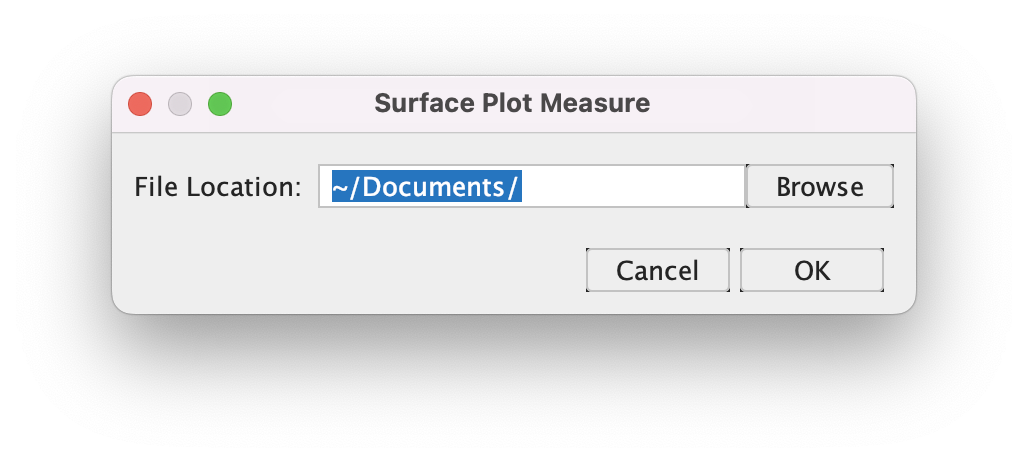
\includegraphics[width=3in]{images/spmeasuregui.png}
\caption{This simple GUI, reminiscent of previous examples, which asks only for the file directory that should be analyzed and will process all of the images matching the parameters in that directory. It selects specifically files that match the file naming pattern of surface plots and should be used directly after the previous script.}
% Provide a label so we can cross\hyp{}reference it from the tex
\label{figure:spmeasuregui}
\end{figure}

\begin{code}
\caption{An R script to capture the maximum point along the profile generated by the previous scripts and then calculate the area under the curve to compare different biological groups to one another.}
\label{blinder}

\inputminted[breaklines,frame=single,fontsize=\small]{r}{source/surface_plot_analysis.R}

\end{code}

This R script takes the CSV format output from FIJI/ImageJ and processes it by finding the maximum value along the curve and using that as the peak relative fluorescence intensity for that X position and then calculates the area under the curve across a defined interval. For instance, the middle 50\% of the cell can be defined as "central" and the outer 25\% can be defined is "distal" and these values normalized to one another and then compared across different experimental groups. It was found that BLaER1 cells infected with \textit{M. tuberculosis} expressing ancestral \textit{esxM} had less distal localization of ARPC2, suggesting that this bacterial effector was altering actin dynamics in these cells via modulation of ARPC2, a finding consistent with previous observations of macrophage from \textit{Arpc2\textsuperscript{-/-}} mice \citep{Rotty2017}.

\section{py-LaRoMe}\label{larome}

The original purpose of LaRoMe (\url{https://github.com/BIOP/ijp-LaRoMe}) is to extract various features from images and is distributed as an ImageJ plugin. However, like many FIJI/ImageJ plugins, the design of LaRoMe is purely operational. In my attempts to utilize CellProfiler \citep{Carpenter2006, Kamentsky2011, McQuin2018, Stirling2021} to automate capture of various details about the THP-1 macrophages from \autoref{thp1inca} and \autoref{thp1lenti}, I wished to incorporate LaRoMe into Python pipelines to increase my throughput of analysis. This, however proved challenging based on the original design of the plugins, as they did not accept an image as an argument and expected to use the currently active image window.

I therefore completely rewrote these plugins explicitly so that they would accept an image as the primary argument, which allows for easy integration into looping structures. In the process, the entire plugin was translated from Java to Python. It is hoped that in the future, these code bases can be reconciled so that the existing distribution of LaRoMe, managed by BIOP, can incorporate both the excellent GUI options already existing and allow for interfacing through scripts for high-throughput applications.

\begin{code}
\caption{A Python translation of the FIJI function ``Label image to ROIs'' from LaRoMe. This function allows the user to take images generated from CellProfiler and convert them into a set of regions of interest in the ROI Manager.}
\label{l2r}

\inputminted[breaklines,frame=single,fontsize=\small]{python}{source/labelsToROIs.py}

\end{code}

\autoref{l2r} allows the user to convert a labeled set of images, for instanced from CellProfiler \citep{Carpenter2006, Kamentsky2011, Stirling2021, McQuin2018} into a set of discrete regions of interest in the ROI Manager within FIJI. This allows for interesting layers of quantitation and segmentation that are otherwise difficult to perform within FIJI due to its difficulty in understanding the RGB layering in the TIFF files produced by CellProfiler. While this work ultimately did not bear much fruit, these approaches seem like they could be broadly useful for others in the future who are trying to do high-throughput, high-content data extraction from labeled images within a larger pipeline. The original implementation is more user-friendly in many ways, but this implementation is, in my opinion, more flexible and with an easier to understand API.

\begin{code}
\caption{A Python translation of the FIJI function ``ROIs to label image'' from LaRoMe. This allows the user to use a set of ROIs to regenerate a label image, useful for creating masks on existing images and comparing areas between different channels.}
\label{r2l}

\inputminted[breaklines,frame=single,fontsize=\small]{python}{source/ROIsTolabels.py}

\end{code}

\autoref{r2l} essentially performs the opposite operation to that performed by \autoref{l2r}. It can use a list of ROIs to generate a new image containing all of the uniquely labeled points and determines the bit-depth of the image based on the number of unique points required. This can be useful in the process of translating multiple labeled images onto one another as well as in integrating labels from multiple processing modalities.

\begin{code}
\caption{A Python translation of the FIJI function ``ROIs to Measurement Image''. This combines the a defined set of ROIs (probably from labelsToROIs.py) and a raw image and generates an image that graphically represents measurements such as area or circularity.}
\label{r2m}

\inputminted[breaklines,frame=single,fontsize=\small]{python}{source/ROIsToMap.py}

\end{code}

The last function in the original LaRoMe transforms a set of ROIs into an image that graphically represents various qualities of the source image. This allows the user to transform a more basic segmented image into ROIs and then use those to measure various aspects of the image from which the ROIs were sourced; this recombines the data from labeled images with the primary data from which it was sourced to generate useful measurements, including the area of fluorescence within the ROI, the relative circularity, the minimum or maximum fluorescence intensity, and more. This utility warrants further exploration going forward in attempting to quantify major aspects of tissue culture immunofluorescence imaging; a more optimized pipeline could likely extract more useful data from the images I already have of various correspondences between NFAT nuclear localization and VEGFA production.

The rewrite allows all of these commands to be strung together to process arbitrary numbers of images all at once and, with intelligent file naming, it should be possible to go from CellProfiler-derived label images to meaningful quantitation of various aspects of the raw images across entire directories of image sets. ``ROIs to Measurement Image'' should probably have an optional GUI similar to the original wrapped around its commands, but I would refer those interested to simply use the original LaRoMe as this implementation and the original are at feature parity.

\section[Experimental Blinding via a Single-Click Command Line Interface]{Experimental Blinding via a Single-Click Command Line Interface\footnote{Implementation from \citet{Brewer2022}, original conception from \citet{Salter2016}.}}\label{blinders}

\begin{code}
\caption{A script to conduct computational filename blinding from the command line written in Python.}
\label{blinder}

\inputminted[breaklines,frame=single,fontsize=\small]{python}{source/renamer.py}

\end{code}

In the process of data collection (especially image acquisition), the experimenter will typically assign each file a logical name indicative of what it contains. However, these file names are also a critical breakdown in analytical blinding and ways to avoid this are essential to prevent the introduction of excess experimenter bias into the process of analysis. This problem is clearly widespread, but solutions are difficult to come by. Individuals can have labmates or others to rename folders or files to obfuscate their contents, but this has the danger of the human element -- it would not be that difficult to lose track of any alterations and make subsequent quantitation worthless. Thus, a computationally robust method is required. 

\citet{Salter2016} saw this issue and elegantly addressed it through a Perl script \citep{Wall2000}. The author generated a script that would allow you to provide a single argument -- a folder -- and have the contents renamed and output a keyfile. This implementation was excellent and used throughout my work, but as time passed, I found it lacking in two major areas: recursion and the ability to undo the renaming. I thus generated a Python implementation that was able to (optionally) recursively move through subdirectories, would provide the exact file path as the original name of the file (useful for feeding into R or FIJI), and came with the ability to provide a folder and keyfile and name all the files back to the original name. In my opinion, these features make for a more complete blinding solution and will hopefully be adopted more widely by users looking to reduce their experimental bias.

This script can be used by first making it executable:

\begin{code}
\begin{minted}{bash}
chmod +x ./renamer.py
\end{minted}
\end{code}

And then calling it by:

\begin{code}
\begin{minted}{bash}
./renamer.py [function] [file directory to rename] [--r]
\end{minted}
\end{code}

Where the "--r" argument is either left absent (for no recursion) or is provided "\hyp{}\hyp{}r" for folder recursion through all non-hidden subdirectories. False is the default for safety. This is a reasonably user-friendly option via the command line is should make experimental blinding much easier. The function is either ``blindrename'' or ``unblind'' and the directory can be provided as a naked string (that is, no ``'' required).

Being written in Python, a GUI could probably be created that would allow this to be even more friendly to the technologically na\"{i}ve user. This would be a relatively modest undertaking and is probably worth considering in the future; this would also allow for more effective cross-platform distribution as compiled binaries.

\section[User-Friendly Analysis of RNA Sequencing Data using Kallisto/Sleuth in a Python Environment]{User-Friendly Analysis of RNA Sequencing Data using Kallisto/Sleuth in a Python Environment\footnote{Taken and expanded from personal contributions to \fullcite{Saelens2022}.}}\label{rnaseq}

While an old technology today, the analysis of RNA sequencing data still unfairly remains a challenge for the technologically na\"{i}ve researcher. To ameliorate part of this problem, in the course of the work in \citet{Saelens2022}, I developed a set of pipelines for the analysis of RNAseq data using a combination of Kallisto and Sleuth, a pair of analysis and visualization applications that utilize pseudoalignment to calculate read counts and then display them in a Shiny application via R \citep{Pimentel2017}.

Conducting this portion of the work required acquainting myself with a number of commonly used computational tools, including cmake and a deeper knowledge of Python and how that can translate into generating a broadly useful cross-platform tool to analyze complex sequencing data. Doing so also required interfacing with FTP and other networking functions and navigating server directories to fetch reference cDNA from Ensembl.

While these were originally implemented as two parallel scripts, one for bacteria and the other for eukaryotes, they have since been consolidated into a single all-purpose script that requests different input based on what is available. The issue with bacterial analysis is that Ensembl has discontinued generating bioMarts for bacterial genomes and has adopted an unpredictable folder structure for fetching these files via FTP. Thus, the user will have to provide the reference transcriptome of their bacterial strain of choice, which can generally be acquired from species-specific databases (Mycobrowser being the notable one here) or from the set of available strains on NCBI or Ensembl. Nonetheless, this should offer a guided experience in the command line to the analysis of RNA sequencing data and provide output that can then be analyzed using either DESeq2 or Sleuth.

\begin{code}
\caption{A guided command line application for the analysis of bulk RNA-seq data using Kallisto.}
\label{blinder}

\inputminted[breaklines,frame=single,fontsize=\small]{python}{source/allKallisto.py}

\end{code}

This script automates many of the most confusing steps for end users by providing an FTP backend to, whenever possible, fetch the needed files aside from the .FASTQ files from the sequencer. Additionally, the use of Kallisto over more traditional alignment methods like STAR or Bowtie allows this to be trivially run on any modern computer without requiring the user to interface with a computing cluster, which is a relatively steep learning curve for many. Kallisto has other advantages as it is much faster and also more accurate than other alignment methods thanks to its pseudoalignment strategy versus more traditional, computationally intensive find-and-match approaches. Kallisto is also robust to unprocessed .FASTQ files, allowing the user to, in many cases, skip adapter trimming and other preprocessing steps. While there is still a place for STAR and HISAT alignments for \textit{de novo} transcript discovery, in most instances, Kallisto will suffice for the task. 

\begin{code}
\caption{Pipeline for the visualization of Kallisto-aligned RNA seq data using Sleuth. This version supports both eukaryotes and bacteria, albeit through two distinct methods of gathering gene lists.}
\label{blinder}

\inputminted[breaklines,frame=single,fontsize=\small]{r}{source/sleuther.R}

\end{code}

Due to policy changes by Ensembl, retrieving pre-packaged marts for bacterial genomes is now impossible on the grounds that the number of bacterial strains has outgrowth Ensembl's ability to provide these marts. Despite the difficulties this creates for finding reference gene lists for even the most common bacterial species (including even \textit{Escherichia coli}), this can be subverted by converting gene lists available from species-specific repositories into a mart-like object that can then be utilized for the downstream steps. No user wants to look at a list of Ensembl IDs after quantitation, and so provision of common gene names is an important component of any analysis. This analysis pipeline was generates specifically for \textit{Mycobacterium tuberculosis}, but could easily be modified to support almost any species.

The logic for fetching and processing bioMarts remains in the script, for use with eukaryotic species. As many of the later steps converge, the user can choose to run particular sets of lines based on their organism. Future versions might wrap some GUI elements or starting booleans to only execute the appropriate commands when needed, but in my experience, it is possible to get a new user working with this script with minimal overall effort.

\section{Bacterial Burden Analysis by Fluorescence Intensity in a Semi-Automated Manner with a User-Friendly Graphical Interface}

One of the major routine tasks in the field of zebrafish-\textit{M. marinum} host-pathogen interactions is the quantitation of the total bacterial burden per larva. While it has been well established that the integrated fluorescence intensity of the image corresponds well to the colony forming units of bacteria present, the larval zebrafish has particular challenges. Many of these are attributable to autofluorescence from the yolk and pigment cells or the physical background of the imaging surface, but it is important to avoid catching these in the quantitation as these can vary greatly from fish to fish and are difficult to subtract \textit{post hoc}. However, through clever approaches to image pre-processing it is possible to eliminate these sources of misquantitation and streamline analysis to minimize user intervention.

\begin{code}
\caption{This graphical user interface allows for automatic background subtraction from images of \textit{M. marinum}-infected larval zebrafish and then quantitation of the remaining signal above a manually set threshold that captures as much of the true signal as possible.}
\label{burden}

\inputminted[breaklines,frame=single,fontsize=\small]{python}{source/burdenMeasurer.py}

\end{code}

This graphical user interface facilitates automatic processing of arbitrary numbers of images at once by allowing users to select various parameters to test for appropriateness in their particular experiment (\autoref{figure:burdengui}). The underlying logic will automatically create Z projections if applicable and then use those for subsequent analysis. Users are encouraged to select a subset of images to start and the computational thresholds are used to capture any objects over a certain size for background removal, which will typically only capture the yolk and any background fluorescence. This approach also allows for more generous manual thresholds to be selected for quantitation, an issue that often arises in manual approaches to fluorescence quantitation due to the need to accommodate this autofluorescence. 

\begin{figure}
\centering
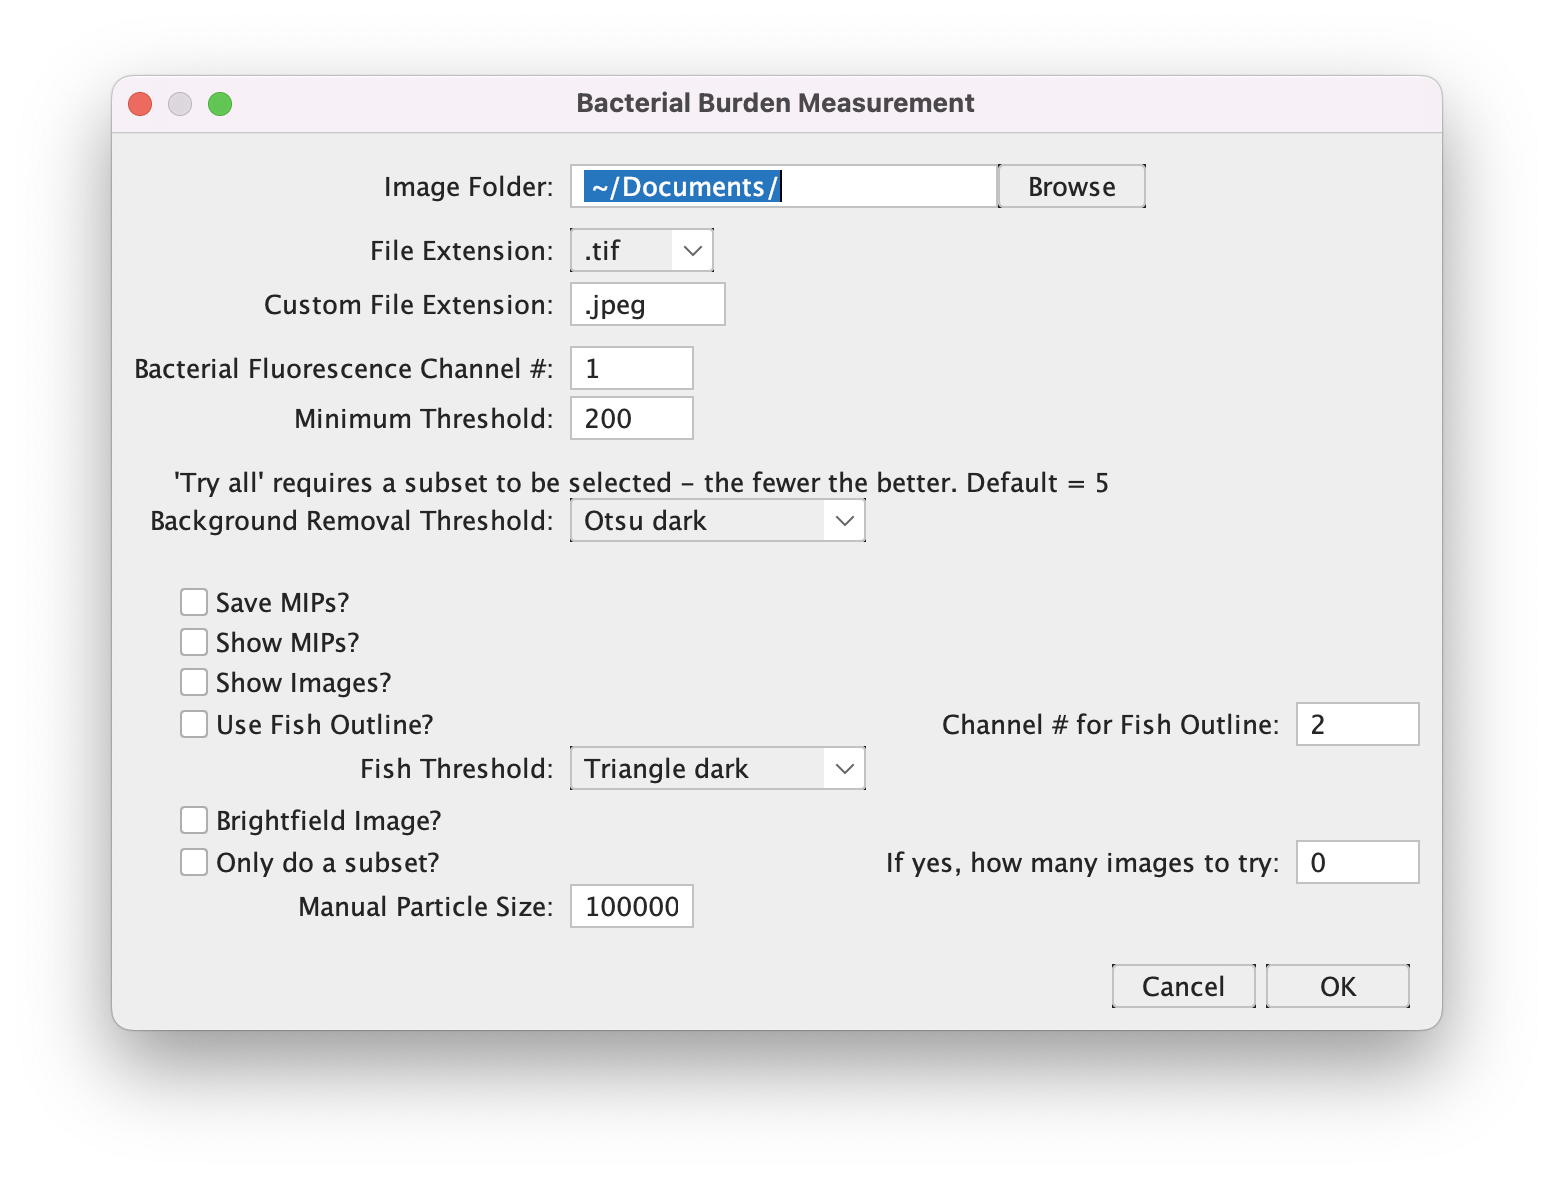
\includegraphics[width=\textwidth]{images/burden_gui.png}
\caption{This graphical user interface guides the user through providing all of the parameters needed to measure burden from a set of larval zebrafish images. All of these parameters require some tweaking by the user, but allows for subsetting to try different combinations to optimize burden measurements within a single experiment.}
% Provide a label so we can cross\hyp{}reference it from the tex
\label{figure:burdengui}
\end{figure}

It is my hope that this application, after further beta testing and refinement can supplant these manual approaches and replace them with something that free researcher time to conduct more experiments rather than spend many hours drawing circles around zebrafish in order to measure the bacterial burden of these fish. Additionally, this could in principle to adapted to measuring other aspects of zebrafish biology, from macrophage clustering to transcriptional reporter signals. The elegance of this approach is that it utilizes open-source and well-defined mechanisms for measuring signal over noise through the implementation of the automatic thresholds and wraps a set of utility functions within an interface that avoids the need for the end user to write burdensome macros to accomplish the same goal. This approach, after a minutes-long period of optimizing is able to measure the burden of thousands of larvae in mere minutes. The output can then be spot-checked for accuracy, as in a small subset of the larvae parts of the background may not be perfectly removed and these can then be reprocessed either manually or with altered parameters. 


